\documentclass[a4paper]{article}
\usepackage{tikz}
\usepackage[landscape]{geometry}
\usetikzlibrary{positioning}


\begin{document}

\section{This is your input string:}
\vspace*{2cm}

\begin{center}
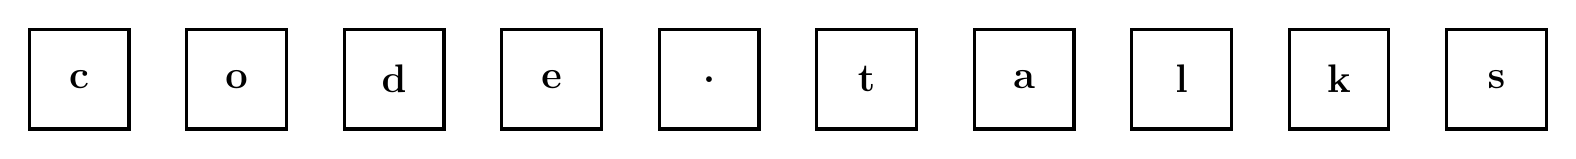
\begin{tikzpicture}
\node[rectangle, draw=black, very thick, inner sep=8pt, minimum size=3\baselineskip] (c) at (0, 0) {\Large\textbf{c}};
\node[rectangle, draw=black, very thick, inner sep=8pt, minimum size=3\baselineskip] (o) at (2, 0) {\Large\textbf{o}};
\node[rectangle, draw=black, very thick, inner sep=8pt, minimum size=3\baselineskip] (d) at (4, 0) {\Large\textbf{d}};
\node[rectangle, draw=black, very thick, inner sep=8pt, minimum size=3\baselineskip] (e) at (6, 0) {\Large\textbf{e}};
\node[rectangle, draw=black, very thick, inner sep=8pt, minimum size=3\baselineskip] (.) at (8, 0) {\Large\textbf{.}};
\node[rectangle, draw=black, very thick, inner sep=8pt, minimum size=3\baselineskip] (t) at (10, 0) {\Large\textbf{t}};
\node[rectangle, draw=black, very thick, inner sep=8pt, minimum size=3\baselineskip] (a) at (12, 0) {\Large\textbf{a}};
\node[rectangle, draw=black, very thick, inner sep=8pt, minimum size=3\baselineskip] (l) at (14, 0) {\Large\textbf{l}};
\node[rectangle, draw=black, very thick, inner sep=8pt, minimum size=3\baselineskip] (k) at (16, 0) {\Large\textbf{k}};
\node[rectangle, draw=black, very thick, inner sep=8pt, minimum size=3\baselineskip] (s) at (18, 0) {\Large\textbf{s}};


\end{tikzpicture}
\end{center}

\vspace*{2cm}
\section{Print this document (single-page, two-sided) and cut out each letter above.}

%\vspace*{2cm}
\section{Now glue your cut-out letters into these boxes, according to the number on the back:}

\begin{center}
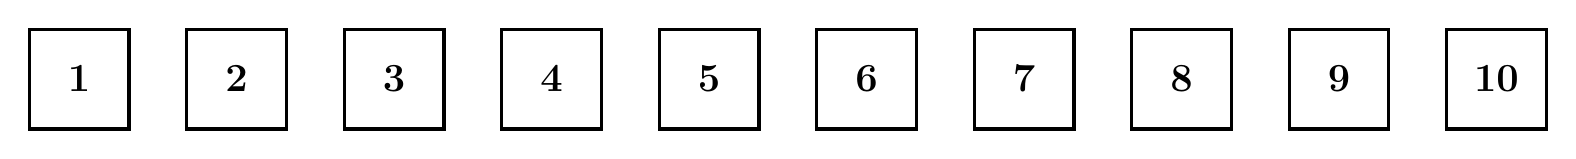
\begin{tikzpicture}
\node[rectangle, draw=black, very thick, inner sep=8pt, minimum size=3\baselineskip] (1) at (0, 0) {\Large\textbf{1}};
\node[rectangle, draw=black, very thick, inner sep=8pt, minimum size=3\baselineskip] (2) at (2, 0) {\Large\textbf{2}};
\node[rectangle, draw=black, very thick, inner sep=8pt, minimum size=3\baselineskip] (3) at (4, 0) {\Large\textbf{3}};
\node[rectangle, draw=black, very thick, inner sep=8pt, minimum size=3\baselineskip] (4) at (6, 0) {\Large\textbf{4}};
\node[rectangle, draw=black, very thick, inner sep=8pt, minimum size=3\baselineskip] (5) at (8, 0) {\Large\textbf{5}};
\node[rectangle, draw=black, very thick, inner sep=8pt, minimum size=3\baselineskip] (6) at (10, 0) {\Large\textbf{6}};
\node[rectangle, draw=black, very thick, inner sep=8pt, minimum size=3\baselineskip] (7) at (12, 0) {\Large\textbf{7}};
\node[rectangle, draw=black, very thick, inner sep=8pt, minimum size=3\baselineskip] (8) at (14, 0) {\Large\textbf{8}};
\node[rectangle, draw=black, very thick, inner sep=8pt, minimum size=3\baselineskip] (9) at (16, 0) {\Large\textbf{9}};
\node[rectangle, draw=black, very thick, inner sep=8pt, minimum size=3\baselineskip] (10) at (18, 0) {\Large\textbf{10}};

\end{tikzpicture}
\end{center}
\pagebreak

\section{These numbers tell you which letter goes where.}
\vspace*{2cm}

\begin{center}
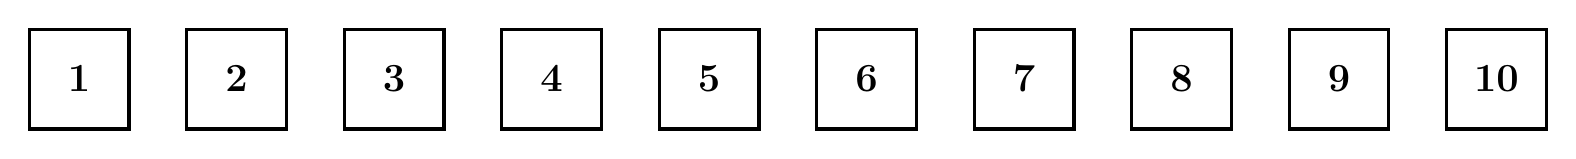
\begin{tikzpicture}
\node[rectangle, draw=black, very thick, inner sep=8pt, minimum size=3\baselineskip] (1) at (0, 0) {\Large\textbf{1}};
\node[rectangle, draw=black, very thick, inner sep=8pt, minimum size=3\baselineskip] (2) at (2, 0) {\Large\textbf{2}};
\node[rectangle, draw=black, very thick, inner sep=8pt, minimum size=3\baselineskip] (3) at (4, 0) {\Large\textbf{3}};
\node[rectangle, draw=black, very thick, inner sep=8pt, minimum size=3\baselineskip] (4) at (6, 0) {\Large\textbf{4}};
\node[rectangle, draw=black, very thick, inner sep=8pt, minimum size=3\baselineskip] (5) at (8, 0) {\Large\textbf{5}};
\node[rectangle, draw=black, very thick, inner sep=8pt, minimum size=3\baselineskip] (6) at (10, 0) {\Large\textbf{6}};
\node[rectangle, draw=black, very thick, inner sep=8pt, minimum size=3\baselineskip] (7) at (12, 0) {\Large\textbf{7}};
\node[rectangle, draw=black, very thick, inner sep=8pt, minimum size=3\baselineskip] (8) at (14, 0) {\Large\textbf{8}};
\node[rectangle, draw=black, very thick, inner sep=8pt, minimum size=3\baselineskip] (9) at (16, 0) {\Large\textbf{9}};
\node[rectangle, draw=black, very thick, inner sep=8pt, minimum size=3\baselineskip] (10) at (18, 0) {\Large\textbf{10}};

\end{tikzpicture}

\end{center}
\end{document}
